\section{Preprocess and data analysis}
\subsection{Data Collection}
As shown by figure~\ref{fig:sysdesign}, our analysis pipeline starts from the plan, log, and system performance data collection.

\stitle{Query plan parsing}
As shown in section~\ref{sec:background}, in Hive, an execution plan is described as a text file involving hundreds to thousands of lines of operations. We parse this file first and generate a directed acyclic graph with the node as the logic vertex and the edge as the data dependencies.

\stitle{Execution log and system performance processing}
Since the Hadoop execution logs are collected with the tedious system log, we locate the records of interest by detecting the keywords from the pre-defined keyword set and then parse these logs and extract the information.
Several important information is saved to the local file, including the task id, the logic vertices corresponding to the tasks, the temporal information(start time, duration) of tasks, the temporal information of steps in a task, etc. 

\subsection{Data Modeling}

\begin{figure}[t]
	\centering
	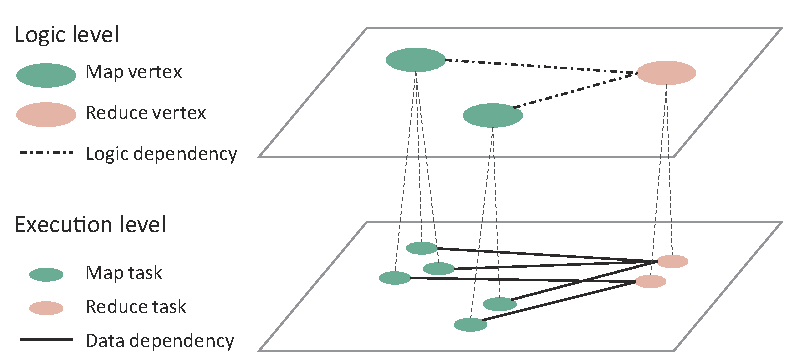
\includegraphics[width=0.42\textwidth]{figures/model/datamodel.pdf}
	\vspace{-3mm}
	\caption{Two-level temporal graph.}
	\label{fig:model}
	\vspace{-3mm}
\end{figure}

The data we collected from backend can be modeled as a temporal graph with two levels: the logic-level and execution-level, which is shown as the figure~\ref{fig:model}. 

As discussed in section~\ref{sec:background}, the logic level graph indicates the DAG extracted from the execution plan, denoted by $\mathbb{G}_L = (\mathbb{V}_L, \mathbb{D}_L)$, where $\mathbb{V}_L$ is the logic vertex set and the $\mathbb{D}_L$ is logic dependency set between the vertices. The execution-level graph denotes the $\mathbb{G}_E = (\mathbb{T}_E, \mathbb{D}_E)$, where $\mathbb{T}_E$ denotes the set of tasks executed by the the physical machines and $\mathbb{D}_E$ indicates the data dependency set between tasks. 
If a task $t \in \mathbb{T}_E$ is an physical instance of vertex $v \in \mathbb{V}_L$, we describe this relationship as the form $t \to v$. We also adopt the this description for the relationship between logic dependency $d_L \in \mathbb{D}_L$ and data dependency $d_E \in \mathbb{D}_E$ such as $d_e \to d_L$. Moreover, we use $P(v) = \{t|\forall t \to v\}$ to indicate all tasks which are the physical instances of $\mathbb{V}_L$. 
A map task $t$ has five steps indicating as an array: $S=<s_{init}, s_{input}, s_{proc}, s_{sink}, s_{spill}>$ and a reduce task have five steps $S=<s_{init}, s_{shuffle}, s_{proc}, s_{sink}, s_{spill}>$. Each step can be modeled by a pair of attributes $<st, d>$ which denotes the start time and duration. Notice that the different steps of the same task may have overlap in time.

According to section~\ref{sec:background}, each task can be modeled as a sequence of attributes: $t:=<st, d, v, m, S_E>$, where $st$, $d$ and $v$ indicate the \textit{start time}, \textit{duration} and logic vertex of task $t$.  $m$ is the machine executes this task and $S_T$ is the corresponding steps. We use $t.attr$ to indicate the $attr$ of $t$.

The vertex can be modeled as triplet: $v:=<st, d, S_L>$. The start time of $v$ is $v.st=min(\{t.st|t \in P(v)\})$, the duration of vertex $e$ is $v.d=v.st+max(\{(v.st+v.d)|t \in P(v) \})$. The steps $S_L=$ $\{d_{init}, d_{input}, d_{proc}, d_{sink}, d_{spill}\}$ or $\{d_{init}, d_{shuffle}, d_{proc}, d_{sink}, d_{spill}\}$ according to the types, and with a given $v$, $d.attr = sum(\{s.attr| s\in S_L\})$ where $attr \in \{init, input, shuffle, proc, sink, spill\}$. 